
\documentclass[journal,12pt,twocolumn]{IEEEtran}
\usepackage{graphicx}
\graphicspath{{./figs/}}{}
\title{
Matrix-Lines
}
\author{Kukunuri Sampath Govardhan}
\begin{document}
\maketitle
\tableofcontents
\begin{abstract}
This document shows how to find equation of a line passing trough a point (2,2) and cutting off intercepts on the axes whose sum is 9 using python.
\end{abstract}
\section{Problem Statement}
Find equation of a line passing trough a point (2,2) and cutting off intercepts on the axes whose sum is 9.\\
\section{Construction}
\begin{figure}[h]
    \centering
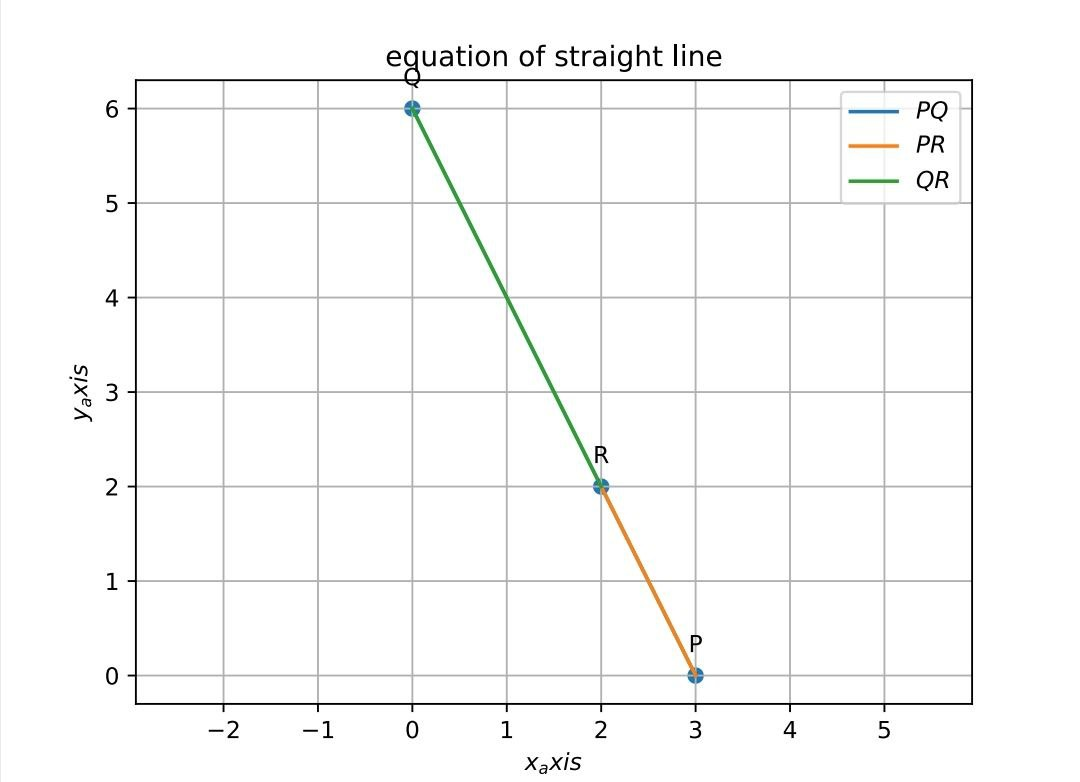
\includegraphics[width=\columnwidth]{figs/assign4.png}
    \caption{Equation of the Straight Line}
    \label{fig:my_label}
\end{figure}

\begin{table}[h]
    \centering
    \begin{tabular}{|c|c|c|}
       \hline
       \textbf{Symbol}&\textbf{Value}&\textbf{Description}  \\
       \hline
        P & (a,0) & Point on X-axis\\
        \hline
        Q & (0,b) & Point on Y-axis\\
        \hline
        R & (2,2) & Given Point \\
        \hline
        a+b & 9 & Given Condition\\
        \hline
    \end{tabular}
    \caption{Parameters}
    \label{tab:my_label}
\end{table}


\section{Solution}
Given that resultant line passes through point(2,2) and intercepts on axes whose sum is 9 (let x intercept is P (a,0) and y intercept is Q (0,b) therefore, a+b=9 ) so, b=9-a  \\
\\
Let P=(a,0),Q=(0,9-a),R=(2,2)\\
\\
Equation of line is \textbf{$n^{T}$X = c} it can also be written as \textbf{$X^{T}$n = c}\\
\\
Now we have 3 points which lies on same line so,\\
$[a$ $0]n = c$ -------eq1  Equation of line through P\\
$[0$ $9-a]n = c$ -------eq2 Equation ofline through Q\\
Now eq1+eq2,\\
$[a$ $9-a]n = 2c$ ------eq3 \\
$[2$ $2]n = c$ ------eq4 Equation of line through R\\
 \\
 From eq3 and eq4 we can find normal vector n,\\
 \\
 $[$$[a$ $9-a]$,$[2$ $2]$$]n$ = c$[2$ $1]$\\
 \\
 Therefore, n = $[$$[a$ $9-a]$,$[2$ $2]$$]^{-1}$. c.$[2$ $1]$\\
 \\
 n = $[3a-9$ $-2]. c/$(4a-18)\\
 \\
 Now eq4 can be expressed as,\\
 \\
  $[3a-9$ $-2]$.$[2$ $2]$.c/(4a-18) = c\\
  \\
  By solving this equation we get a=2,thus b=9-a=7\\
  \\
  by substuting a in n, finally\\
  \\
  n = $[0.3$ $0.2]. c$
  \\
The Resultant Equation of line is \textbf{$n^{T}$X = c} \\
\\
i.e,    \textbf{$[0.3$ $0.2]. X$ = 1}\\
\\
\section{Software}
Download the following code using, \\
\begin{table}[h]
    \centering
    \begin{tabular}{|c|}
    \hline \\
         svn co https://github.com/\\mygit-sampath-govardhan/fwc-iith-assignments/blob/\\5b65abbf8e5e3c803b1bff8cf4a95092e100de75/\\Assignment-4(Matrices-line)/codes/Assignment4.py  \\
   \hline
    \end{tabular}
\end{table}
\\
Now execute the code \\
\\
\textbf{Python3  Assignment4.py}\\
\section{Conclusion}
We found the equation of a line passing trough a point
(2,2) and cutting off intercepts on the axes whose
sum is 9.

\end{document}
